\chapter{Resultater} \label{resultat}

I dette afsnit vil det endelige resultat af det færdigudviklede detekteringssystem blive beskrevet. Detekteringssystemet blev testet i accepttesten og resultaterne for testen vil blive præsenteret i dette kapitel. 

I accepttesten blev de tre Use Cases testet. Henholdsvis Use Case 1: Tilkobling af system, Use Case 2: Detektering og Use Case 3: Kalibrering. Ydermere blev ikke-funktionelle krav til detekteringssystemet testet løbende med Use Casene. Use Case 1 forløb som forventet og Use Casen opnåede det ønskede resultat, hvormed systemet blev tilkoblet korrekt.  

Til at teste Use Case 2, blev det valgt at teste alle fire scenarier, for derved at validere detekteringssystemets performance. Detekteringssystemet er udviklet på baggrund af egenskaberne ved højtryksballonen Atlas$^\circledR$ Gold, 22 mm. Det var til accepttestens udførsel ikke muligt at fremskaffe denne type ballon og testen blev derfor udført med True\texttrademark \ Dilatation Balloon, 22 mm, \cite{DatabladTrue}. Detekteringsalgoritmen er indstillet til et threshold på 4, da det ved udvikling af algoritmen viste sig, at dette threshold detekterer alle fraktureringer i alle scenarier. Da Use Case 2 skulle udføres, viste det sig, at der ved hurtig inflatering ikke konsekvent blev detekteret en frakturering, da amplituden ikke oversteg et threshold på 4, se algoritmegraf på Figur \ref{alg2}. Ydeligere ses det, at inflateringsstøjen ikke nærmer sig 2. 

\begin{figure}[H]
	\centering
	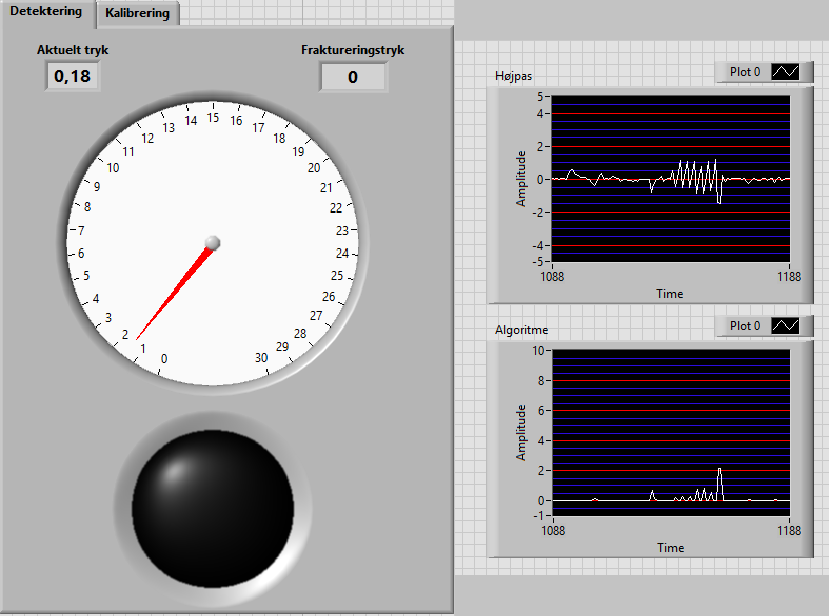
\includegraphics[width=0.7\textwidth]{Figure/alg2}
	\caption{Accepttest ved hurtig inflatering hvor fraktur ikke detekteres, da amplituden ikke overstiger threshold på 4}
    \label{alg2}
\end{figure}

Scenariet som ses på Figur \ref{alg2}, forekom ved gentagende sprængninger. På baggrund af dette, blev det derfor valgt at ændre detekteringsalgoritmens threshold til 2 og udføre accepttesten ved denne værdi. Det vurderes, at denne forskel muligvis kan skyldes egenskaberne ved den nye ballon og Use Casen blev derfor godkendt, trods denne ændring. 

På Figur \ref{detektering1} ses detekterings GUI, hvor Use Case 2 er fuldendt og det ønskede resultat er opnået. Det ses på den grønne lampe, at en frakturering er blevet detekteret, samt det ses, at fraktureringen skete ved et tryk på 10,26 atm. Ydeligere præsenterer GUI'en det aktuelle tryk på 1,51 atm, hvilket passer overens med det tryk, som kan aflæses på gaugen. 

\begin{figure}[H]
	\centering
	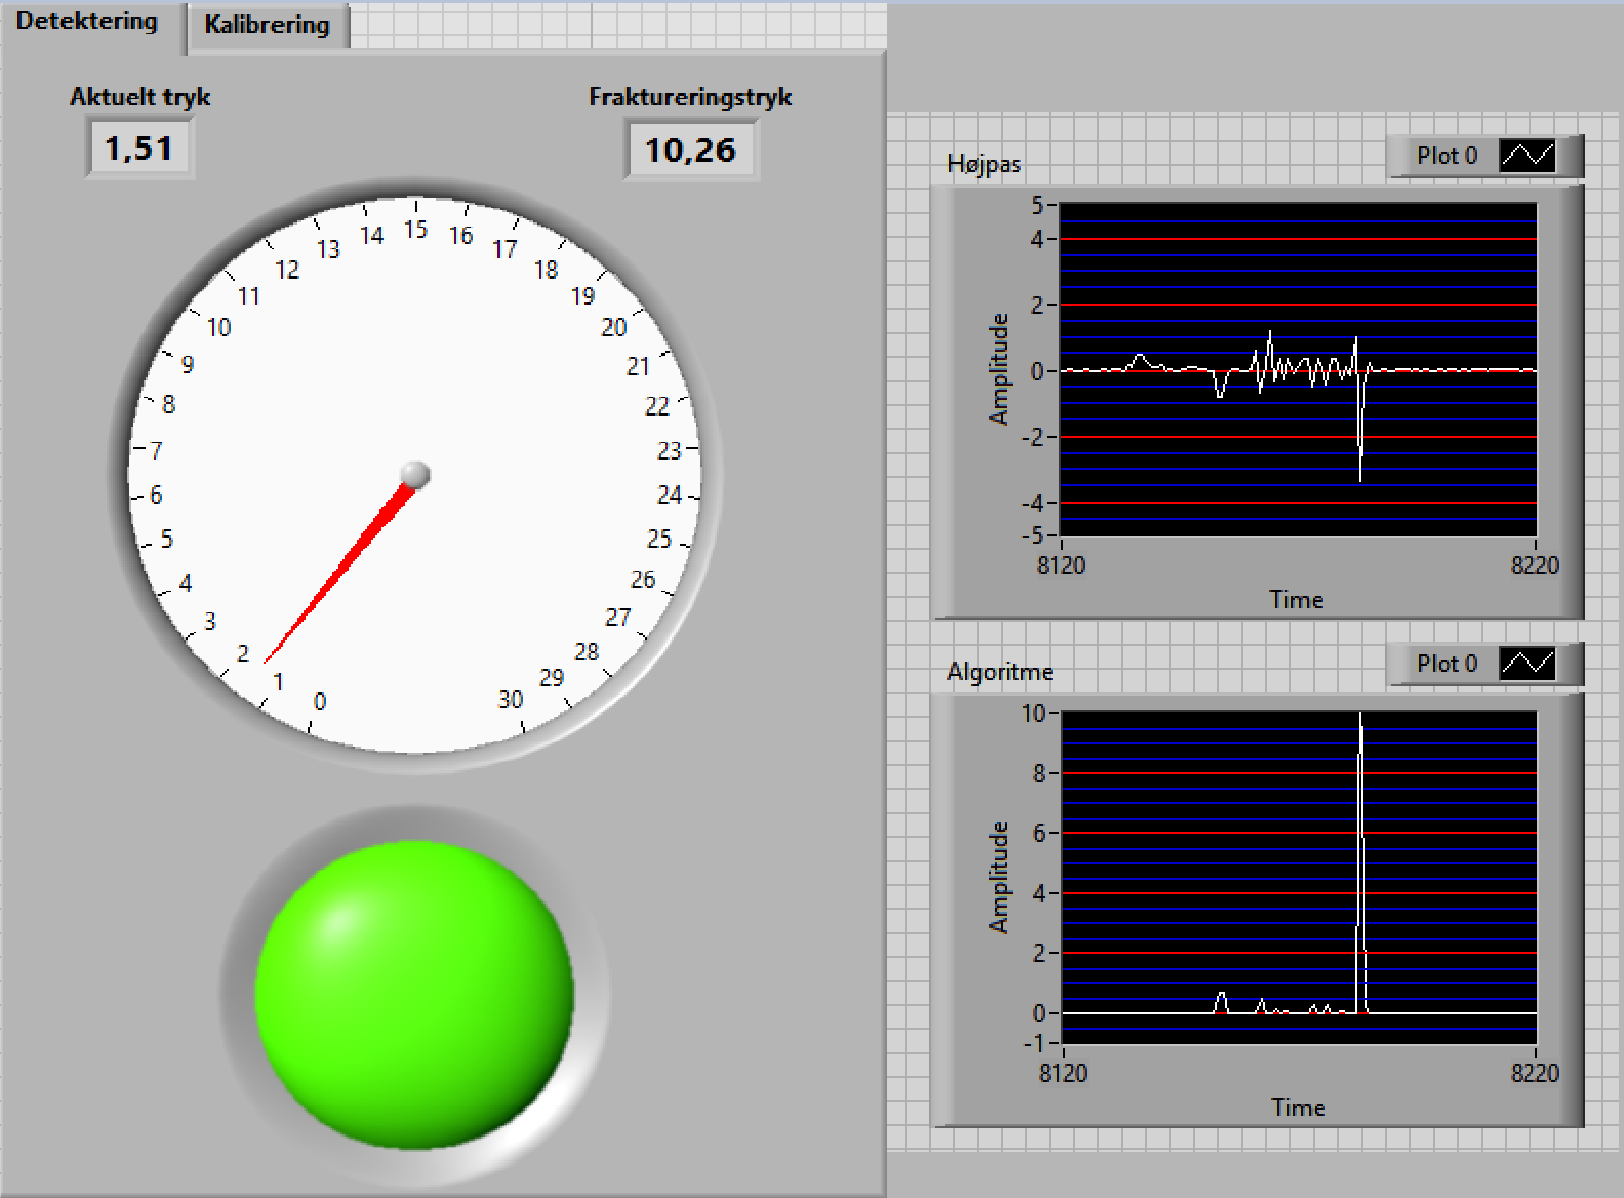
\includegraphics[width=0.7\textwidth]{Figure/detekteirng}
	\caption{Detekterings GUI, hvor en frakturering er blevet detekteret}
    \label{detektering1}
\end{figure}

På Figur \ref{kaliGUI}, ses kalibrerings GUI. Her ses kalibrerings tabellen, hvor default trykværdier er angivet, samt der er mulighed for at indskrive den aktulle spænding. Ved 5 atm ses det, at den aktuelle spænding er 1,63 V, hvilket er indskrevet i tabellen. Use Case 3 afsluttes ved at åbne detekterings fanen, hvormed detekteringssystemet er kalibreret. For at validere kalibreringen, blev der påført et tryk på 5 atm via inflatoren. På detekterings GUI'en kunne der aflæses et tryk på 5 atm, hvormed det verificeres, at kalibreringen er udført korrekt. Dermed blev Use Case 3 accepteret.  

\begin{figure}[H]
	\centering
	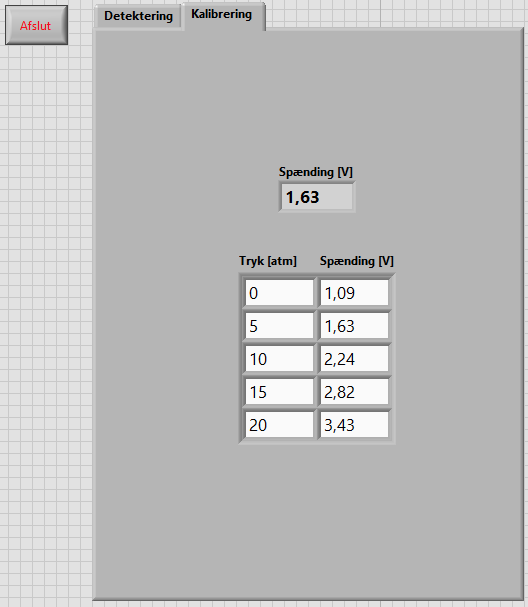
\includegraphics[width=0.7\textwidth]{Figure/kaliGUI}
	\caption{Kalibrerings GUI}
    \label{kaliGUI}
\end{figure}








